Laravel rende semplice la connesione al database e successiva esecuzione delle query attaverso l'\gls{ORM}, passando per il query builder. Una volta configurato il \gls{database} il sistema è pronto per eseguire le query tramite la Facade DB fornito da \gls{Laravel}. Tale classe fornisce svariati metodi di commando come, select, update, insert, ecc..
Nei diagrammi di sequenza viene illustrata l'interazione tra il \gls{database} e il recupero dei parametri, richiesti dai services del front-end. Le associazioni tra richieste e controller sono mappate nel file \textit{routes.php}. Un controller termina la propria esecuzione restituendo al service del front-end un oggetto JSON che contiene:
\begin{itemize}
	\item i parametri corretti se la richiesta va a buon fine ed il metodo preveda il ritorno di essi;
	\item un messaggio di successo nel caso il metodo non preveda il ritorno di alcun paramento(es. salvataggio sul \gls{database});
	\item un messaggio di errore nel caso la richiesta non vada a buon fine.
\end{itemize}

\subsubsection{Richieste REST}
Si mostrano i diagrammi di sequenza di alcune chiamate REST che effettua il sistema per meglio specificarne il funzionamento.

\paragraph{3.2.1.1 GET user/:username/project}\mbox{}\\
Il diagramma sottostante illustra le operazioni necessarie alla ricerca e restituzione della lista di tutti i progetti relativi ad un utente. Dal \textit{service} del front-end arriva una richiesta Http che viene instradata alla classe \textbf{ProjectController} mediante il file \textit{routes.php}. Il ProjectController recupera l'username dell'utente autenticato tramite una invocazione della funzione ausiliaria \textit{Auth::user()}, fornita da \textit{Laravel}, e lo confronta con il parametro \textit{username} passato nella richiesta per verificare la correttezza di tale richiesta. Una volta recuperato l'utente autenticato invoca il metodo \textit{projects()} che ritorna la lista di tutti i progetti relativi a tale utente.

	\begin{figure}[h]
		\centering
		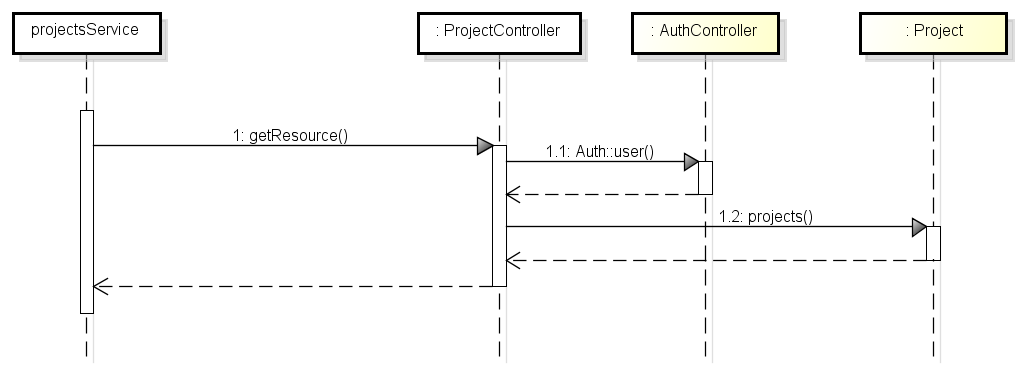
\includegraphics[width=0.7\linewidth]{img/GET_projects}
		\caption[GET user/:username/project]{GET user/:username/project}
		\label{fig:GET user/:username/project}
	\end{figure}

\newpage
\paragraph{3.2.1.2 POST user/:username/project}\mbox{}\\
Il diagramma sottostante illustra le operazioni necessarie alla creazione di un nuovo progetto. Dal \textit{service} del front-end arriva una richiesta Http che viene instradata alla classe \textbf{ProjectController} mediante il file \textit{routes.php}. Il ProjectController recupera l'username dell'utente autenticato tramite una invocazione della funzione ausiliaria \textit{Auth::user()}, fornita da \textit{Laravel}, crea un nuovo progetto tramite il costruttore di default e gli assegna i valori contenuti nella richiesta Http. La creazione del progetto lancia un evento di tipo \textbf{ProjectWasCreated} che crea una istanza di questa classe. Tale classe a sua volta, collegata a due \textit{Listeners}, istanzia una classe di tipo \textbf{PresentationCreate} che crea una nuova presentazione all'interno del progetto appena creato e una classe di tipo \textbf{SlideCreate} che crea la prima \gls{slide}, di anteprima, della presentazione appena creata.

	\begin{figure}[h]
		\centering
		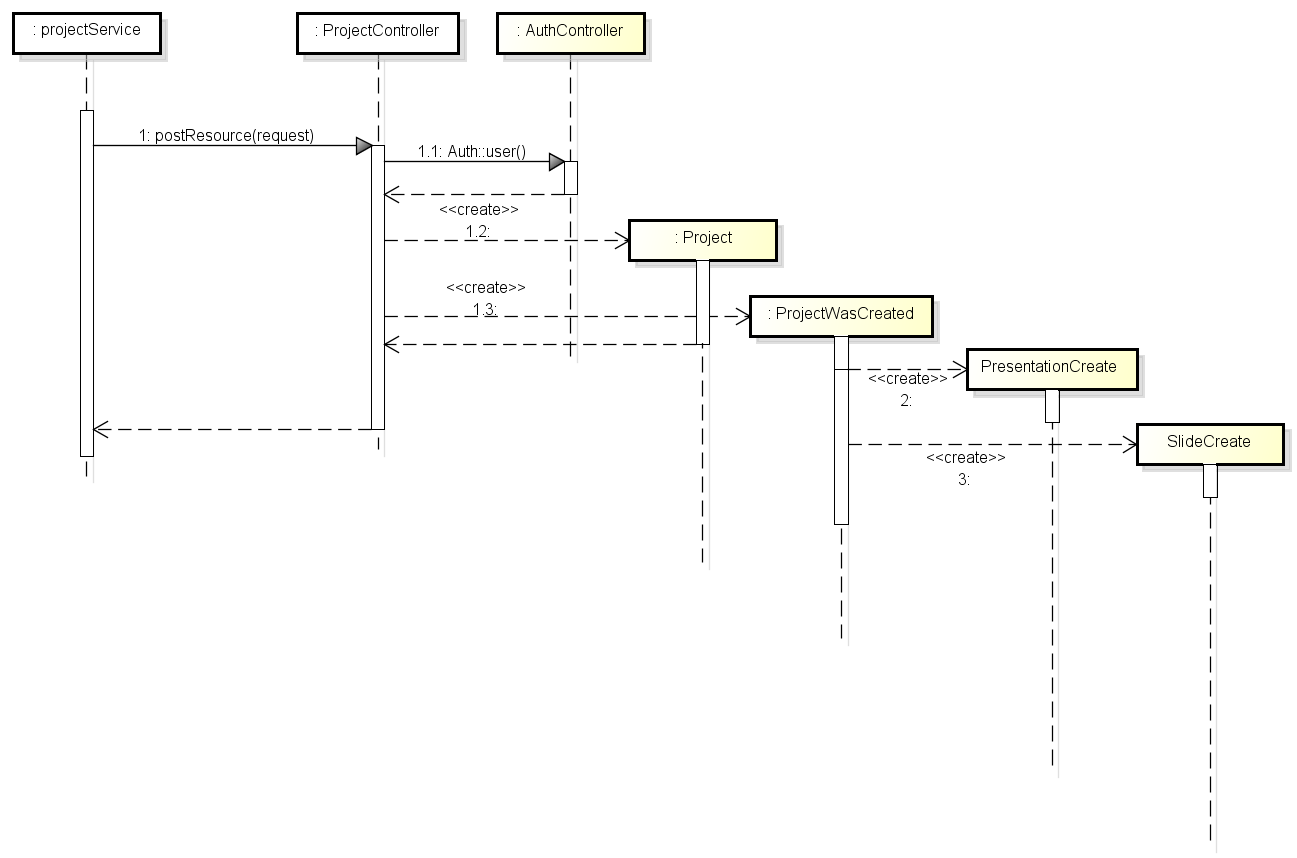
\includegraphics[width=0.6\linewidth]{img/POST_project}
		\caption[POST user/:username/project]{POST user/:username/project}
		\label{fig:POST user/:username/project}
	\end{figure}

\newpage

\paragraph{3.2.1.3 PUT user/:username/project/:projectID}\mbox{}\\
Il diagramma sottostante illustra le operazioni necessarie all'aggiornamento dei dati di un progetto esistente. Dal \textit{service} del front-end arriva una richiesta Http che viene instradata alla classe \textbf{ProjectController} mediante il file \textit{routes.php}. Il ProjectController recupera l'username dell'utente autenticato tramite una invocazione della funzione ausiliaria \textit{Auth::user()}, fornita da \textit{Laravel}, su tale utente invoca il metodo \textit{projects()} che ritorna la lista dei progetti dell'utente. Su tale lista viene invocato il metodo \textit{find(projectID)} che ritorna il progetto da aggiornare. Successivamente utilizza i parametri contenuti nella richiesta Http per aggiornare i dati del progetto su cui viene invocato il metodo \textit{save} che salva il progetto aggiornato nel database.

	\begin{figure}[h]
		\centering
		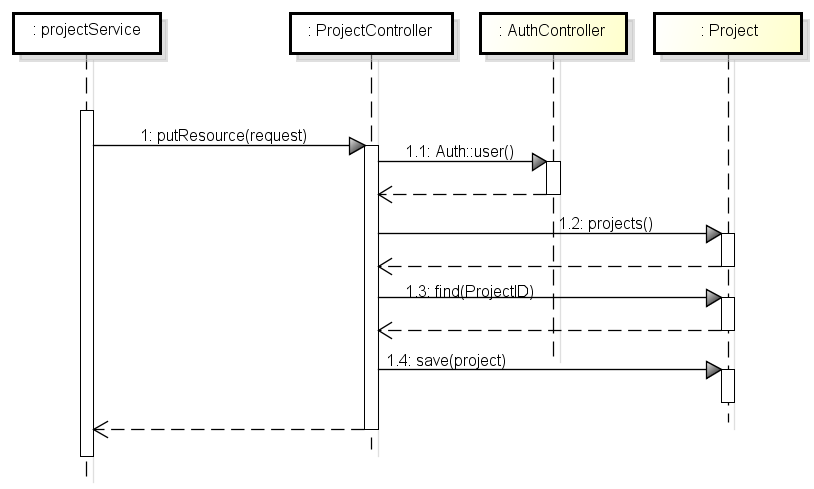
\includegraphics[width=0.6\linewidth]{img/PUT_project}
		\caption[PUT user/:username/project/:projectID]{PUT user/:username/project/:projectID}
		\label{fig:PUT user/:username/project/projectID}
	\end{figure}

\paragraph{3.2.1.4 DELETE user/:username/project/:projectID}\mbox{}\\
Il diagramma sottostante illustra le operazioni necessarie alla cancellazione di un progetto esistente. Dal \textit{service} del front-end arriva una richiesta Http che viene instradata alla classe \textbf{ProjectController} mediante il file \textit{routes.php}. Il ProjectController recupera l'username dell'utente autenticato tramite una invocazione della funzione ausiliaria \textit{Auth::user()}, fornita da \textit{Laravel}, su tale utente invoca il metodo \textit{projects()} che ritorna la lista dei progetti dell'utente. Su tale lista viene invocato il metodo \textit{find(projectID)} che ritorna il progetto da eliminare. Su tale progetto viene invocato il metodo \textit{delete()} che rimuove il progetto dal database.

	\begin{figure}[h]
		\centering
		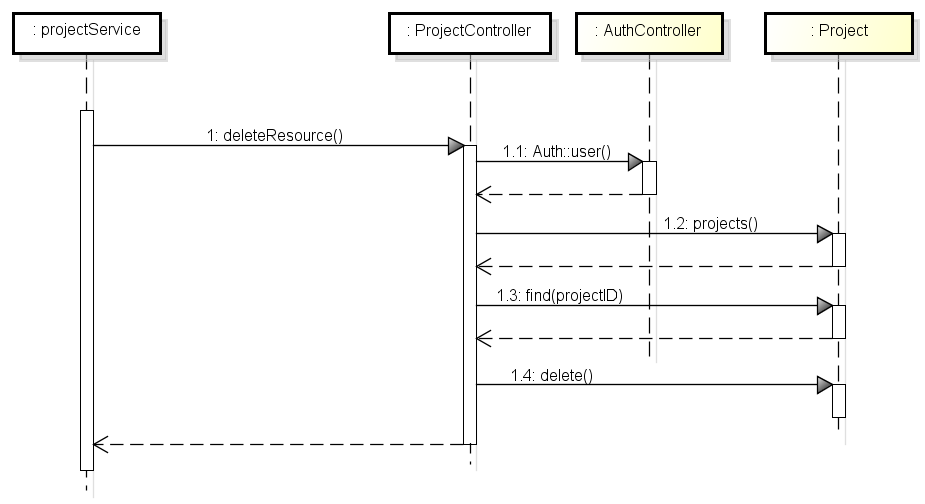
\includegraphics[width=0.6\linewidth]{img/DELETE_project}
		\caption[DELETE user/:username/project/:projectID]{DELETE user/:username/project/:projectID}
		\label{fig:DELETE user/:username/project/:projectID}
	\end{figure}
	
\newpage

\paragraph{3.2.1.5 PUT user/:username/project/:projectID/presentation/:presentationID}\mbox{}\\
Il diagramma sottostante illustra le operazioni necessarie all'aggiornamento dei dati di una presentazione. Dal \textit{service} del front-end arriva una richiesta Http che viene instradata alla classe \textbf{PresentationController} mediante il file \textit{routes.php}. Il PresentationController recupera l'username dell'utente autenticato tramite una invocazione della funzione ausiliaria \textit{Auth::user()}, fornita da \textit{Laravel}, su tale utente invoca il metodo \textit{projects()} che ritorna la lista dei progetti dell'utente. Su tale lista viene invocato il metodo \textit{find(projectID)} che ritorna il progetto da cui aggiornare la presentazione. Su tale progetto viene invocato il metodo \textit{presentation()} che ritorna la presentazione, vengono aggiornati i suoi campi tramite i valori contenuti nella richiesta Http, ed infine invocato il metodo \textit{save()} che salva la presentazione nel database.

\begin{figure}[h]
	\centering
	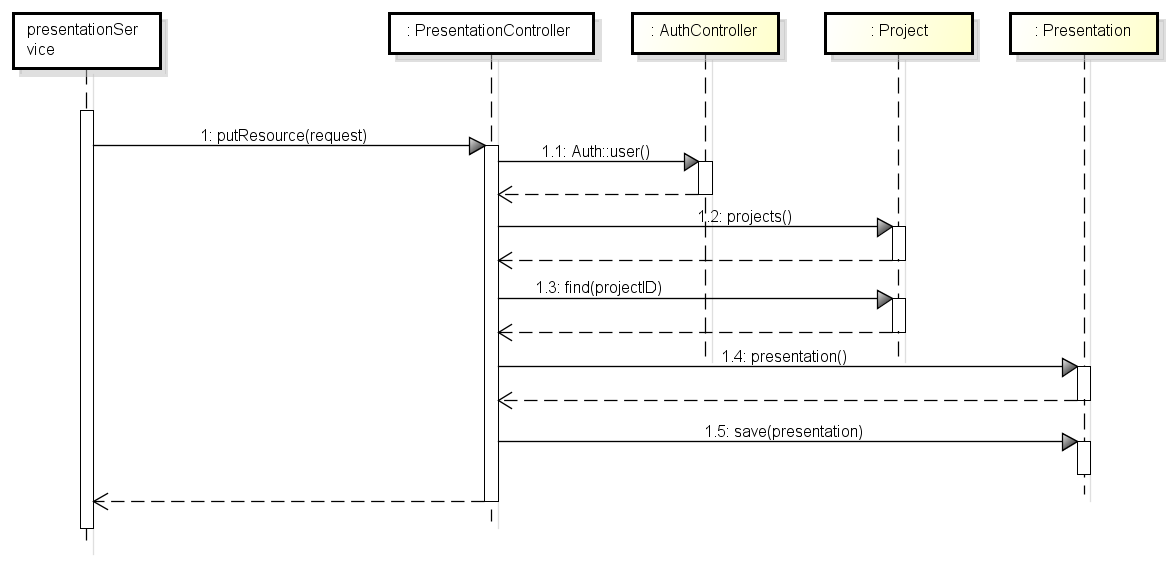
\includegraphics[width=0.6\linewidth]{img/PUTpresentation}
	\caption[PUT user/:username/project/:projectID/presentation/:presentationID]{PUT user/:username/project/:projectID/presentation/:presentationID}
	\label{fig:PUT user/:username/project/:projectID/presentation/:presentationID}
\end{figure}

\paragraph{3.2.1.5 DELETE user/:username/project/:projectID/presentation/:presentationID}\mbox{}\\
Il diagramma sottostante illustra le operazioni necessarie alla cancellazione della presentazione associata ad un progetto esistente. Dal \textit{service} del front-end arriva una richiesta Http che viene instradata alla classe \textbf{PresentationController} mediante il file \textit{routes.php}. Il PresentationController recupera l'username dell'utente autenticato tramite una invocazione della funzione ausiliaria \textit{Auth::user()}, fornita da \textit{Laravel}, su tale utente invoca il metodo \textit{projects()} che ritorna la lista dei progetti dell'utente. Su tale lista viene invocato il metodo \textit{find(projectID)} che ritorna il progetto da cui eliminare la presentazione. Su tale progetto viene invocato il metodo \textit{presentation()} che ritorna la presentazione su cui viene invocato il metodo \textit{delete()} che la rimuove dal database.

\begin{figure}[h]
	\centering
	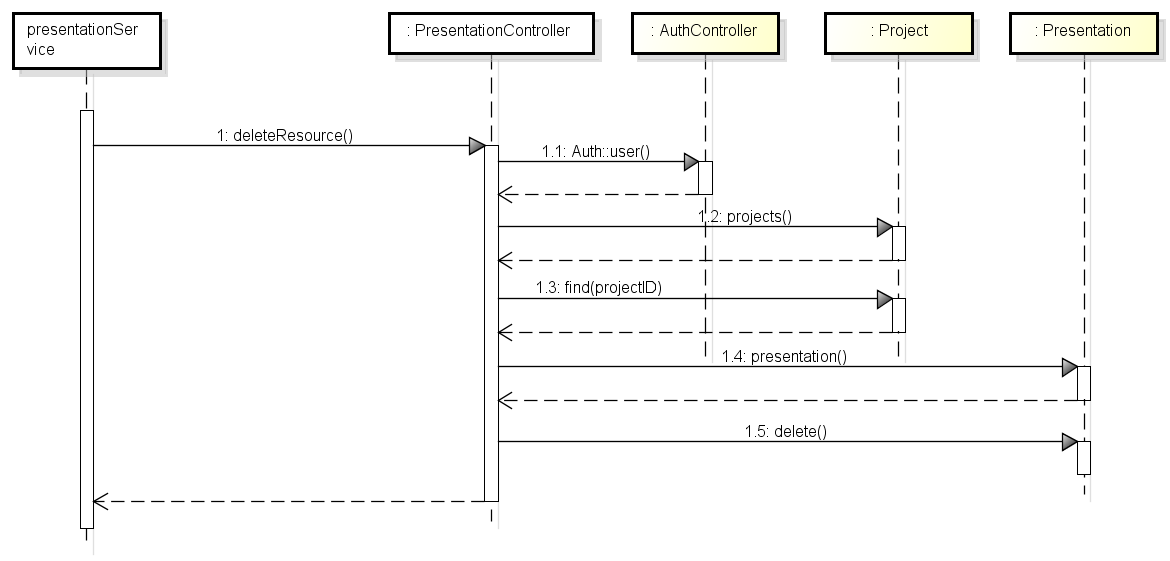
\includegraphics[width=0.6\linewidth]{img/DELETEpresentation}
	\caption[DELETE user/:username/project/:projectID/presentation/:presentationID]{DELETE user/:username/project/:projectID/presentation/:presentationID}
	\label{fig:DELETE user/:username/project/:projectID/presentation/presentationID}
\end{figure}
